\documentclass{article}

\usepackage[UTF8]{ctex} % 加载ctex宏包,并指定UTF8编码
\usepackage{url}
\usepackage{booktabs}
\usepackage{geometry}
\usepackage{amsmath} % 其他你可能需要的宏包
\usepackage{graphicx} % 其他你可能需要的宏包

\geometry{margin=2.5cm}

\title{情感分析的基础实验}
\author{李牧之}
\date{\today}

\begin{document}

\maketitle 

\section{Introduction}
情感分析,又称为意见挖掘,旨在识别和提取文本数据中所表达的情感、观点和主观信息,将文本内容分类到积极、消极等情感类别中。广泛应用于商业、社交媒体等需要理解用户意见的领域。本文基于python和IMDB电影评论数据集,运用词袋(BoW)、TF-IDF、深度学习、预训练模型、大型语言模型调用等方法进行基础实验,并对模型性能进行简单对比评估。

\section{Dataset}

\subsection{数据集信息}
IMDB电影评论数据集,包含5万条英语原始评论,每条评论含有真实的情感倾向标签,并且被平均分为了积极与消极两部分。
\\数据集中前十条数据:
\begin{center}
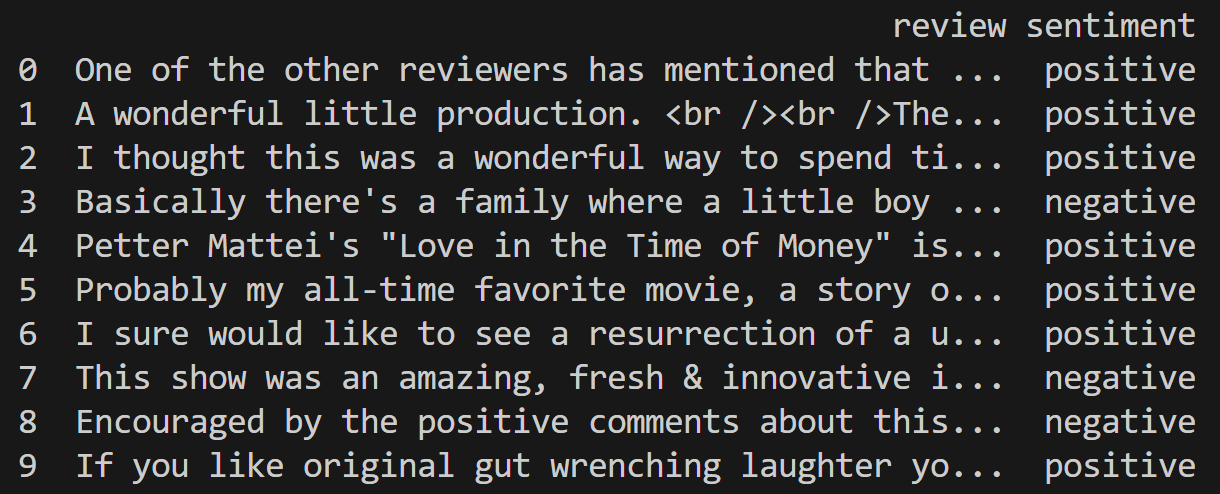
\includegraphics[scale=0.3]{PNG2.png}
\end{center}
\\下载链接:

\url{https://www.kaggle.com/lakshmi25npathi/imdb-dataset-of-50k-movie-reviews}

\subsection{数据处理}
\subsubsection{数据清洗 Data Cleaning}
对于数据集中的数据,我们仅考虑其中的词汇,因此要去除特殊符号、数字等;同时将大小写归一化。
\subsubsection{停用词过滤 Stop Words Removal}
停用词(Stop Words)是指在自然语言文本中出现频率很高但对文本意义贡献很小的词,将这些词语过滤掉。
\subsubsection{词干提取 Stemming}
将一个词语的不同形式还原成词干,通过去除前后缀来进行,将具有相同基本意义的词语归一化。
\subsubsection{深度学习方法所需要的进一步数据处理}\label{sssec:2.2.4}
深度学习方法不需要进行停用词过滤以及词干提取。在数据清理之后,进行词汇表的创建,每一个词语赋予独特的索引值,将评论文本转换为一串整数。大约共有92K的单词,其中前10K的单词就可以覆盖文中约95\%的单词。所以仅考虑前10K的单词,并将单一评论长度限制为500词,短于500词用特殊索引填充,长于500词则只考虑前500词进行截取。
\begin{center}
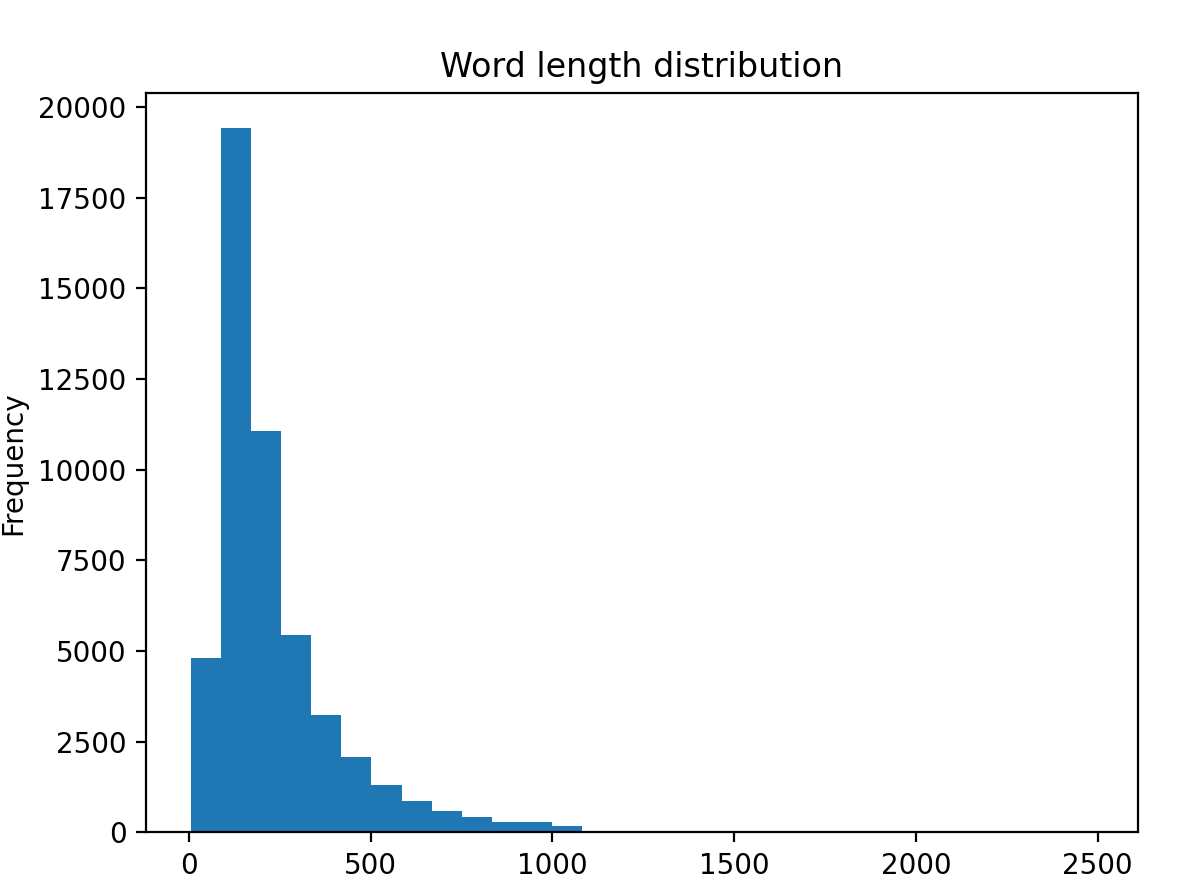
\includegraphics[scale=0.7]{PNG1.png}
\end{center}

\section{Methods}
\subsection{Bag of Words} \label{3.1}
词袋模型(Bag of Words,简称BoW)是自然语言处理中最基础、最核心的文本表示方法之一。词袋模型将文档视为无序的词汇集合,忽略语法和语序,仅统计每个词语出现的频率,将文本转化为数值向量。其基本步骤如下:1)文本预处理,进行数据清洗、停用词过滤、词干提取以及分词;2)构建词汇表,收集测试集所有文档中的所有不重复的词语,构成词汇表,单词总数称为词汇表大小(Vocabulary Size);3)文本向量化,将每篇文档根据各单词出现的频次结合词汇表表示为词频向量(Bag of Words Vector),向量维度为词汇表大小,向量中的每个位置都对应着词汇表中的一个词,该位置的值为该单词出现的频次。例如,文档1:"John likes to watch movies. Mary likes movies too."文档2:"Mary also likes to watch football games."则构建词汇表为["john", "likes", "to", "watch", "movies", "mary", "too", "also", "football", "games"],长度为10,则文档1的词频向量为[1, 2, 1, 1, 2, 1, 1, 0, 0, 0],文档2的词频向量为[0, 1, 1, 1, 0, 1, 0, 1, 1, 1]。

在词袋模型中,为了更好的提取复合短语的语义信息,可以使用n-grams,截取连续的n个单词作为词汇表中的一个单词,即词频向量中的一个维度。

\subsection{TF-IDF} \label{3.2}
TF-IDF是对于词袋模型中词频向量生成方法的改进,该方法的核心思想为:一个单词的重要性与它在当前文档中的出现次数正相关,与它在所有文档中的出现次数负相关。其基本步骤如下:1)文本预处理;2)构建词汇表;3)文本向量化,将每篇文档表示为词汇向量,向量的每个位置对应词汇表中的一个词,该位置的值为该词语的TF-IDF值。
\begin{equation}
    TFIDF(t,d,D)=TF(t,d)*IDF(t,D) \label{eq1}
\end{equation}
\begin{equation}
    TF(t,d)=\text{单词t在文档d中的出现频次} \label{eq2}
\end{equation}
\begin{equation}
    IDF(t,D)=\log(\frac{1+N}{1+DF(t)})+1 \label{eq3}
\end{equation}

给定总文档库D,文档总数为N,单词t,某一文档d,DF(t)为包含单词t的文档数。根据公式\eqref{eq1}\eqref{eq2}\eqref{eq3}计算出单词t在文档d中的TF-IDF值。IDF(Inverse Document Frequency,逆文档频率)有多种计算方式,本文采用sklearn库中TfidfVectorizer函数的计算公式,在分子和分母上加1以避免某些词在所有文档中都不出现的情况,否则可能出现分母为0的错误。此外,sklearn库中的TfidfVectorizer函数还对最终的TF-IDF向量进行了L2范数归一化,即对于每一个文档的向量,所有值的平方和为1。

TF-IDF模型中也可以使用n-grams方法以更好提取复合短语的语义信息。

\subsection{Logistic Regression}
逻辑回归(Logistic Regression)是一种用于解决二元分类问题的统计学习方法,尽管名字中含有“回归”,但它实际上是一种分类算法。其核心任务是根据输入的特征向量预测某个事件发生的概率,并根据这个概率将数据点归类到两个类别中的一个。在本文研究的情感分析任务中,输入的特征向量即为\ref{3.1},\ref{3.2}中的词频向量,两个类别即为"Positive""Negative"两种情感极性。

逻辑回归的核心工作原理如下:1)对输入的特征向量\textbf{x}进行加权求和,计算出一个线性得分z,即公式\eqref{eq4},其中$\boldsymbol{\theta}$是模型需要通过训练来学习的权重;2)将线性得分z传入Sigmoid函数,将z映射成[0,1]之间的一个概率值,即公式\eqref{eq5},若P大于等于0.5,则模型预测其类别为1,若P小于0.5,则模型预测其类型为0。
\begin{equation}
    z=\theta_0+\sum_{i=1}^n\theta_ix_i \label{eq4}
\end{equation}
\begin{equation}
    P(y=1|\textbf{x})=\frac{1}{1+e^{-z}} \label{eq5}
\end{equation}

逻辑回归的训练是一个优化过程,其目标是找到一组最佳的权重,使得模型的预测概率尽可能接近真实标签。训练过程主要依赖梯度下降算法来最小化交叉熵损失(Cross-Entropy Loss),即公式\eqref{eq6},其中m为样本总数,$y^{(i)}$为第i个样本的真实标签,$p(x^{(i)})$为第i个样本输出为1的概率。本文采用sklearn中的LogisticRegression模型,初始参数$\boldsymbol{\theta}$会被赋值为不相等的近似为0的随机值,根据梯度下降算法更新参数,即公式\eqref{eq7},其中$\alpha$为学习率,在本文使用的模型中根据L-BFGS优化算法调整。多次更新参数之后损失函数的值不再显著下降,此时认为模型已经收敛。此外,sklearn中的LogisticRegression模型默认使用L2正则化,以减缓模型的过拟合现象。
\begin{equation}
    J(\boldsymbol{\theta})=-\frac{1}{m}\sum_{i=1}^m[y^{(i)}\log(p(x^{(i)}))+(1-y^{(i)})\log(1-p(x^{(i)}))] \label{eq6}
\end{equation}
\begin{equation}
    \theta_j:=\theta_j-\alpha\frac{\partial}{\partial\theta_j}J(\boldsymbol{\theta}) \label{eq7}
\end{equation}

\subsection{Linear Support Vector Machine}
线性支持向量机(Linear Support Vector Machine,LSVM)是一种监督学习算法,主要用于解决二分类问题。其核心思想是寻找一个超平面(hyperplane),将不同类别的样本向量分开,并使得该超平面到两边最近的样本(该样本被称为支持向量,Support Vectors)的距离(称为间隔,Margin)最大化。训练完成后,根据输入向量与超平面的位置关系即可确认其输出。我们将标签值定义为$\pm1$,记优化得到的超平面方程为\eqref{eq8},则对于样本向量$\boldsymbol{x_i}$,预测规则为\eqref{eq9}。
\begin{equation}
    \boldsymbol{w^Tx}+b=0 \label{eq8}
\end{equation}
\begin{equation}
    f(\boldsymbol{x_i})=sign(\boldsymbol{w^Tx_i}+b) \label{eq9}
\end{equation}

LSVM优化的基本约束条件为\eqref{eq10},即对于正类样本$(y_i=+1)$,要求$\boldsymbol{w^Tx_i}+b\geq+1$;对于负类样本$(y_i=-1)$,要求$\boldsymbol{w^Tx_i}+b\leq-1$,且满足$y_i(\boldsymbol{w^Tx_i}+b)=1$的数据点就是支持向量。优化目标是最大化间隔,数学上容易证明间隔大小为$\frac{2}{\|\boldsymbol{w}\|}$,其中$\|\boldsymbol{w}\|$是向量$\boldsymbol{w}$的L2范数,最大化$\frac{2}{\|\boldsymbol{w}\|}$等价于最小化$\|\boldsymbol{w}\|$,也等价于最小化$\frac{1}{2}{\|\boldsymbol{w}\|}^2$,因此,LSVM的基本优化目标为\eqref{eq11}
\begin{equation}
    y_i(\boldsymbol{w^Tx_i}+b)\geq1 \label{eq10}
\end{equation}
\begin{equation}
    \min_{w,b}\frac{1}{2}{\|\boldsymbol{w}\|}^2 \quad \text{subject to} \quad y_i(\boldsymbol{w^Tx_i}+b)\geq1 \quad \forall x=1 , \cdots , n \label{eq11}
\end{equation}

然而,仅考虑\eqref{eq10}\eqref{eq11}无法解决一些不是完全线性可分的问题,为此,我们引入"软间隔"(Soft Margin),允许一些样本点被错误分类,但会对此进行惩罚。引入松弛变量$\xi_i\geq0$,修改约束条件为\eqref{eq12},如果$\xi_i=0$,表示样本点被正确分类,且位于间隔之外,如果$0<\xi_i<1$,表示样本点被正确分类,但位于间隔之内,如果$\xi_i\geq1$,表示样本点被错误分类。同时,在优化目标中加入对松弛系数的惩罚项,即\eqref{eq13},其中C是惩罚系数,在本文使用的sklearn.svm.LinearSVC模型中默认为1.0。为了最小化总损失,$\xi_i$取满足约束条件的最小值,即$max(0,1-y_i(\boldsymbol{w^Tx_i}+b))$,结合\eqref{eq12}\eqref{eq13},得到最终的目标函数,即带合页损失的软间隔SVM\eqref{eq14}。
\begin{equation}
    y_i(\boldsymbol{w^Tx_i}+b)\geq1-\xi_i \label{eq12}
\end{equation}
\begin{equation}
    \min_{w,b}\frac{1}{2}{\|\boldsymbol{w}\|}^2+C\sum_{i=1}^{n}\xi_i \quad \text{subject to} \quad y_i(\boldsymbol{w^Tx_i}+b)\geq1-\xi_i \label{eq13}
\end{equation}
\begin{equation}
    \min_{w,b}\frac{1}{2}{\|\boldsymbol{w}\|}^2+C\sum_{i=1}^{n}\max(0,1-y_i(\boldsymbol{w^Tx_i}+b)) \label{eq14}
\end{equation}

对于该目标函数,本文使用模型采用序列最小优化算法(Sequential Minimal Optimization,SMO)。

\subsection{Multinomial Naive Bayes}
多项式朴素贝叶斯(Multinomial Naive Bayes, MNB)是一种基于贝叶斯定理专门用于处理离散特征的分类算法,其核心思想"朴素"指的是一个强假设:假设所有特征之间是相互独立的。在情感分析任务中,这意味着文档中某个词的出现与其他词的出现是完全独立的,没有任何关联。多项式朴素贝叶斯算法的基础是贝叶斯定理,即\eqref{eq15},其中$P(C|D)$为后验概率(Posterior Probability),即在文档D出现的情况下属于类别C的概率,为预测时需要求解的目标;$P(D|C)$为似然度(Likelihood),即在类别C出现的情况下,文档D出现的概率,通过训练数据进行计算;$P(C)$为先验概率(Prior Probability),即没有任何信息的情况下一个文档属于类别C的概率;$P(D)$为证据(Evidence),即文档D出现的概率,在分类问题中可被视为常数不予考虑。最终的分类规则是寻找后验概率最大的类别C。
\begin{equation}
    P(C|D)=\frac{P(D|C)P(C)}{P(D)} \label{eq15}
\end{equation}

对于情感分析问题,文档D被表示成为\ref{3.1},\ref{3.2}中的词频向量,例如$\boldsymbol{x}=(x_1,...,x_n)$,其中$n$为词语个数,$x_i$是词语$w_i$在上述方法中对应的取值(出现次数或TF-IDF值)。根据所有特征相互独立的假设,我们可以将后验概率表示为\eqref{eq16},为方便计算,取对数得\eqref{eq17}。由于最后只需比较各类别后验概率的相对大小,可以将\eqref{eq17}取等作为计算结果进行分类。
\begin{equation}
    P(C|D)\propto P(C)\prod_{i=1}^{n}P(w_i|C)^{x_i} \label{eq16}
\end{equation}
\begin{equation}
    \log P(C|D)\propto \log P(C) + \sum_{i=1}^{n}x_i·\log P(w_i|C) \label{eq17}
\end{equation}

训练过程中,利用训练集的数据根据\eqref{eq18}\eqref{eq19}计算先验概率以及各词语的似然度,其中\eqref{eq19}使用了拉普拉斯平滑,$\alpha$为平滑参数,默认值为1.0。预测过程,将词频向量数据带入\eqref{eq17}计算"Positive"和"Negative"对应的后验概率再进行比较,选择较大的类别作为预测结果。
\begin{equation}
    P(C)=\frac{\text{类别C的文档数}}{\text{总文档数}} \label{eq18}
\end{equation}
\begin{equation}
    P(w_i|C)=\frac{\text{类别C文档中词语$w_i$的$x_i$之和}+\alpha}{\text{类别C文档中的$\sum_{j=1}^nx_j$之和}+\alpha · n} \label{eq19}
\end{equation}

\subsection{Multilayer Perception} \label{3.6}
多层感知机(Multilayer Perception,MLP),也被称为全连接神经网络(Fully-connected Neutral Network),是一种经典的深度学习模型,它由多个神经元层组成,其中每一层的神经元都与前一层所有的神经元相连接。在情感分析任务中,MLP的核心任务是通过多个隐藏层增加非线性组合构建一个映射关系,将输入的文档映射为情感标签。

经过\ref{sssec:2.2.4}的数据处理,每条文档被处理为一个长度为500的整数序列,传入输入层(InputLayer)。在嵌入层(Embedding)中,每一个词语被转换称为一个固定大小(本文实验使用的大小为32)的嵌入向量(Embedding Vector),转换过程中的嵌入参数需要通过学习得到,嵌入向量能够捕捉词语之间的语义关系,相似的词语在嵌入空间中具有相似的向量表示,最后嵌入层的输出为二维数据块,经过展平层(Flatten)得到一个一维向量,传入全连接隐藏层(Dense)。隐藏层中使用"ReLU"激活函数,并设有Dropout层,以减缓过拟合现象,输出层采用Sigmoid函数,表示评论为"Positive"标签的可能性,损失函数使用二元交叉熵损失\eqref{eq6},优化器使用Adam。

\subsection{Recurrent Neutral Network}
循环神经网络(Recurrent Neutral Network,RNN)是一种专门用于处理序列数据的神经网络,它引入了循环结构,使得模型能够利用时序信息和上下文信息。RNN按照序列的时间步进行计算,每一个时间步t根据该时间步的输入$\boldsymbol{x_t}$以及上一时间步计算得到的隐藏状态$\boldsymbol{h_{t-1}}$计算得到该时间步的隐藏状态$\boldsymbol{h_t}$,最终输出最后一个时间步的隐藏状态$\boldsymbol{h_n}$或者所有时间步的隐藏状态序列$\boldsymbol{[h_1,...,h_n]}$。本文使用的是Keras库中的SimpleRNN,根据\eqref{eq20}进行计算,其中$\boldsymbol{W_{hh}}$为隐藏状态到隐藏状态的权重矩阵,$\boldsymbol{W_{xh}}$为输入到隐藏状态的权重矩阵,$\boldsymbol{b}$为偏置向量,$\boldsymbol{h_0}$默认值为$\boldsymbol{0}$,$\tanh$是一个非线性的激活函数,可将输入压缩到(-1,1)的范围内。
\begin{equation}
    \boldsymbol{h_t}=\tanh({\boldsymbol{W_{hh}h_{t-1}}}+\boldsymbol{W_{xh}x_t}+\boldsymbol{b}) \label{eq20}
\end{equation}
\begin{equation}
    \tanh(x)=\frac{e^x-e^{-x}}{e^x+e^{-x}} \label{eq21}
\end{equation}

本文在SimpleRNN的基础上使用双向循环层(Bidirectional,RNN),结合了两个独立的RNN,一个从序列的开头向结尾处理,另一个从序列的结尾向开头处理,并将相同时间步的隐藏状态进行拼接,返回值为两个方向最终隐藏状态的拼接。将该拼接向量传入全连接层,经Sigmoid函数激活后进行预测。损失函数使用二元交叉熵损失\eqref{eq6},优化器使用Adam。

\subsection{LSTM}
长短时记忆网络(Long Short Term Memory,LSTM)是一种特殊的RNN,它通过引入"门控机制"(Gating Machanism)来精确控制信息的流动,从而能够有效地学习和记忆长距离的依赖关系。LSTM的核心是一个特殊的单元结构,由细胞状态(Cell State),遗忘门(Forget Gate),输入门(Input Gate),输出门(Output Gate)构成。

一个LSTM单元在时间步t的计算如下:1)遗忘门,决定丢弃哪些信息,它会接收当前输入$\boldsymbol{x_t}$和上一时刻的隐藏状态$\boldsymbol{h_{t-1}}$,根据\eqref{eq22}计算出遗忘向量$\boldsymbol{f_t}$,其中$\sigma$是Sigmoid函数,$\boldsymbol{[h_{t-1},x_t]}$是将两个向量拼接,$\boldsymbol{f_t}$接近0表示遗忘,接近1表示保留。
\begin{equation}
    \boldsymbol{f_t}=\sigma(\boldsymbol{W_f \cdot [h_{t-1},x_t]}+\boldsymbol{b_f}) \label{eq22}
\end{equation}

2)输入门,决定保留哪些信息,首先根据\eqref{eq23}计算输入门向量$\boldsymbol{i_t}$,决定哪些信息需要被更新;再根据\eqref{eq24}计算候选细胞状态$\boldsymbol{\tilde{C_t}}$,创建一个新的候选向量用于更新细胞状态。
\begin{equation}
    \boldsymbol{i_t}=\sigma(\boldsymbol{W_i \cdot [h_{t-1},x_t]}+\boldsymbol{b_i}) \label{eq23}
\end{equation}
\begin{equation}
    \boldsymbol{\tilde{C_t}}=\tanh(\boldsymbol{W_C \cdot [h_{t-1},x_t]}+\boldsymbol{b_C}) \label{eq24}
\end{equation}

3)更新细胞状态,用遗忘向量逐元素乘旧的细胞状态丢弃旧信息,用输入门向量逐元素乘候选细胞状态添加新信息,相加得到新的细胞状态,即\eqref{eq25}
\begin{equation}
    \boldsymbol{C_t}=\boldsymbol{f_t \odot C_{t-1}}+\boldsymbol{i_t \odot \boldsymbol{\tilde{C_t}}} \label{eq25}
\end{equation}

4)输出门,决定最终输出什么内容,根据\eqref{eq26}计算输出们向量$\boldsymbol{o_t}$,决定细胞状态的哪一部分可以输出,根据\eqref{eq27}计算最终隐藏状态$\boldsymbol{h_t}$作为当前时间步的输出以及下一时间步的部分输入。
\begin{equation}
    \boldsymbol{o_t}=\sigma(\boldsymbol{W_o \cdot [h_{t-1},x_t]}+\boldsymbol{b_o}) \label{eq26}
\end{equation}
\begin{equation}
    \boldsymbol{h_t}=\boldsymbol{o_t \odot \tanh(C_t)} \label{eq27}
\end{equation}

本文的实验模型使用双向循环层,结果传入全连接层经Sigmoid函数激活后进行预测。损失函数使用二元交叉熵损失\eqref{eq6},优化器使用Adam。

\subsection{1D CNN}
一维卷积神经网络(1D Convolutional Neural Network,1D CNN)是一种基于卷积运算的神经网络,其核心思想是将文本视为一维序列数据,并使用卷积核(Kernel)在序列上滑动,提取局部特征。每个文档数据经过嵌入层的处理之后转换为嵌入向量的序列,传入卷积层,每个卷积层包含多个卷积核,分别提取不同的局部特征。每个卷积核都是一个小的权重矩阵,在嵌入向量的序列上滑动计算,它会与n个词向量(n是卷积核的大小,默认为3)进行点积,产生新的特征值。每个卷积核在整个序列上滑动完之后,会生成一个一维的特征图。所有的特征图随后被传入池化层,池化层的目的是降维和突出最重要的特征,本文使用的是最大值池化(MaxPooling),在特征图上以固定大小的窗口滑动,并只保留窗口内的最大值。池化结果再次传入卷积层进行卷积,多次循环操作之后,数据被压缩成为更小更抽象的特征向量。将最后一层池化层的输出通过展平层转换为一个一维向量,输入全连接层,经Sigmoid激活后进行预测。损失函数使用二元交叉熵损失\eqref{eq6},优化器使用Adam。

\subsection{BERT \& RoBERTa}
BERT(Bidirectional Encoder Representations from Transformers)是一种预训练语言模型,其核心是Transformer架构中的Encoder部分,利用自注意力机制(Self-Attention Mechanism)来理解词语之间的关系,从而生成高质量的词嵌入。BERT能够同时从左侧和右侧的上下文理解词语,并且在大规模语料库上进行了预训练,学习了丰富的语言知识,包括语法、语义和句法结构。我们无需从头训练,只需要在预训练的BERT模型上进行微调(fine-tuning)。预训练的主要任务为掩码语言模型(MLM)和下一句预测(NSP)。

在使用BERT解决情感分析任务时,我们只需进行简单的数据清洗,去除文档中的网页以及特殊字符,不需要做进一步的数据处理。文档输入首先传入嵌入层,分别进行:1)词嵌入:为词语提供基本的语义信息;2)段嵌入:为模型提供句子段落的信息;3)位置嵌入:使用固定的正弦-余弦函数生成位置向量,提供词语在序列中的位置信息。三者相加,形成一个融合了所有基础信息的最终输入嵌入向量。该序列的嵌入向量表示为一个矩阵$\boldsymbol{X}$,其中每一行$\boldsymbol{x_i}$是第i个词语的嵌入向量,传入Transformer Encoder层。模型使用三个可学习的权重矩阵,将输入矩阵$\boldsymbol{X}$投影到三个不同的向量空间,分别得到查询矩阵$\boldsymbol{Q}$,键矩阵$\boldsymbol{K}$,值矩阵$\boldsymbol{V}$即\eqref{eq28}\eqref{eq29}\eqref{eq30}
\begin{equation}
    \boldsymbol{Q}=\boldsymbol{XW_Q} \label{eq28}
\end{equation}
\begin{equation}
    \boldsymbol{K}=\boldsymbol{XW_K} \label{eq29}
\end{equation}
\begin{equation}
    \boldsymbol{V}=\boldsymbol{XW_V} \label{eq30}
\end{equation}

我们通过计算查询矩阵与键矩阵的点积,来衡量每个词语与其他所有词语的关联程度,即\eqref{eq31},其中$\boldsymbol{QK^T}$是一个$n\times n$的矩阵,其中每个元素(i,j)都是$\boldsymbol{q_i}$与$\boldsymbol{k_j}$的点积,表示第i个词对第j个词的关注度,结果除以键向量维度的平方根$\sqrt{d_k}$防止梯度过大,最后使用softmax函数将注意力分数转换为(0,1)的注意力权重,且每行权重和为1。最后用注意力权重矩阵$\boldsymbol{A}$对值矩阵$\boldsymbol{V}$进行加权求和,即\eqref{eq32}$\boldsymbol{Z}$是自注意力机制的最终输出矩阵,融合了句子中所有词语的信息,并且对更相关的词语给予了更高的权重。再将该矩阵输入多层Transformer Encoder,进一步提取更高级别、更抽象的上下文信息。多次重复后,输出一个最终的向量序列。
\begin{equation}
    \boldsymbol{A}=softmax(\frac{\boldsymbol{QK^T}}{\sqrt{d_k}}) \label{eq31}
\end{equation}
\begin{equation}
    \boldsymbol{Z}=\boldsymbol{AV} \label{eq32}
\end{equation}

在情感分析任务中,我们使用的是BertForSequenceClassification模型,这是一个专门为序列分类任务设计的BERT模型,除了词向量序列,该模型还会在每个序列的开头添加一个特殊标记[CLS],其对应的最终隐藏状态被特别训练,用于聚合整个输入序列的信息。最终向量序列中含有[CLS]标记的向量被传入分类头(一个全连接层),映射到二维,得到模型对积极与消极情感的预测分数,比较大小进行预测。

RoBERTa(Robustly optimized BERT pretraining approach)在BERT的基础上,对预训练方法进行了优化。它在掩码语言模型任务中使用动态掩码,在每次向模型提供数据时,都动态生成新的掩码模式。这意味着一个句子在不同的训练周期中,被遮盖的词语是不同的。它移除了下一句预测任务。它采用了更大的训练数据和批处理大小,以及训练更长时间,取得比BERT更好的性能。

\subsection{Large Language Model}
大语言模型(Large Language Model,LLM)是具有强大的语言理解和推理能力的通用模型。我们通过设计一个清晰、明确的提示(Prompt),将情感分析任务转化为一个自然语言问答任务描述给模型,模型利用其在海量数据中学到的通用语言理解能力,直接对文本进行分析和分类。本文使用的是"qwen-plus"模型。

\section{Experiments}

\subsection{Bags of Words}
使用sklearn库中的CountVectorize实现一个词、一个词+两个词、一个词+两个词+三个词的三种词袋。数据集中前40K的数据用作训练集,后10K数据用作测试集。仅通过训练集中的评论来构建词汇表,且同一词汇表将被应用于测试集。分别使用逻辑回归(Logistic Regression)、线性支持向量机(LSVM)、朴素贝叶斯(NB)进行机器学习。评测指标为准确率(Accuracies)。

\begin{table}[htbp]
    \centering
    \caption{基于词袋实验准确率结果}
    \label{tab:Accuracies of experiments_1}
    \begin{tabular}{lccc} 
        \toprule 
        Methods & Unigrams & Uni+Bigrams & Uni+Bi+Trigrams \\
        \midrule 
        Logistic Regression & 88\% & 90\% & 90\% \\
        LSVM & 86\% & 90\% & 89\% \\
        NB & 85\% & 88\% & 89\% \\
        \bottomrule 
    \end{tabular}
\end{table}

\subsection{TFIDF}
实现一个词、一个词+两个词、一个词+两个词+三个词的三种TF-IDF词袋.数据集中前40K的数据用作训练集,后10K数据用作测试集。分别使用逻辑回归(Logistic Regression)、线性支持向量机(LSVM)、朴素贝叶斯(NB)进行机器学习。评测指标为准确率(Accuracies)。

\begin{table}[htbp]
    \centering
    \caption{基于词频实验准确率结果}
    \label{tab:Accuracies of experiments_2}
    \begin{tabular}{lccc} 
        \toprule 
        Methods & Unigrams & Uni+Bigrams & Uni+Bi+Trigrams \\
        \midrule 
        Logistic Regression & 89\% & 89\% & 88\% \\
        LSVM & 89\% & 90\% & 90\% \\
        NB & 86\% & 89\% & 89\% \\
        \bottomrule 
    \end{tabular}
\end{table}

\subsection{深度学习方法 Deep Learning}
使用\ref{sssec:2.2.4}进一步处理后的数据,应用基于Tensorflow的多层感知机(MLP)、循环神经网络(RNN)、长短时神经网络(LSTM)、1D卷积神经网络(1D CNN)进行深度学习。随机抽取80\%的数据作为训练集,剩余20\%数据作为测试集。评测指标为准确率(Accuracies)。

\begin{table}[htbp]
    \centering
    \caption{深度学习实验准确率结果}
    \label{tab:Accuracies of experiments_3}
    \begin{tabular}{lc} 
        \toprule 
        Methods & Accuracies \\
        \midrule 
        MLP & 87.0\% \\
        RNN & 84.0\% \\
        LSTM & 88.9\% \\
        1D CNN & 89.7\% \\
        \bottomrule 
    \end{tabular}
\end{table}

\subsection{预训练模型以及大模型调用 Pre-trained Models \& LLMs}
使用基于Hugging Face库的BertForSequenceClassification和RobertaForSequenceClassification进行本地微调后训练,随机选取70\%的数据作为训练集,15\%的数据作为验证集,15\%的数据作为测试集。评测指标为准确率(Accuracies)。

调用"qwen-plus"的API,随机选取20\%的数据作为测试集。

\begin{table}[htbp]
    \centering
    \caption{预训练模型以及大模型调用实验准确率结果}
    \label{tab:Accuracies of experiments_4}
    \begin{tabular}{lc} 
        \toprule 
        Methods & Accuracies \\
        \midrule 
        BERT & 91.9\% \\
        RoBERTa & 92.7\% \\
        qwen-plus & 94.5\% \\
        \bottomrule 
    \end{tabular}
\end{table}

\section{Summary}
根据上述实验结果汇总得到表\ref{tab:Accuracies of All_experiments},调用"qwen-plus"大模型具有最高的准确率94.5\%,使用预训练模型进行本地微调也可以达到92\%左右的较高准确率。


\begin{table}[htbp] 
    \centering
    \caption{实验准确率结果汇总}
    \label{tab:Accuracies of All_experiments}
    \begin{tabular}{lc} 
        \toprule 
        Methods & Accuracies \\
        \midrule 
        Logistic Regression with BOW & 90.0\% \\
        LSVM with BOW & 90.0\% \\
        NB with BOW & 89.0\% \\
        Logistic Regression with TFIDF & 89.0\% \\
        LSVM with TFIDF & 90.0\% \\
        NB with TFIDF & 89.0\% \\
        MLP & 87.0\% \\
        RNN & 84.0\% \\
        LSTM & 88.9\% \\
        1D CNN & 89.7\% \\
        BERT & 91.9\% \\
        RoBERTa & 92.7\% \\
        qwen-plus & 94.5\% \\
        \bottomrule 
    \end{tabular}
\end{table}

\section{More Information}

\subsection{References}
1.\url{https://dropsofai.com/sentiment-analysis-with-python-bag-of-words/}

2.\url{https://dropsofai.com/sentiment-analysis-with-python-tfidf-features/}

3.\url{https://dropsofai.com/sentiment-classification-with-deep-learning-rnn-lstm-and-cnn/}

\subsection{Github Link}
\url{https://github.com/GabrielMu2006/Sentiment-Analysis}

\end{document}